\section{Proportional Controller}\label{chap:pController}
A proportional controller can be used to do a first approximation to the behavior of the system in closed loop, knowing that it can not be the final solution for the problem.

As it can be seen in \figref{closedLoopResponse}, the closed loop function has an unstable response when a step reference of 1 rad is required.

\begin{figure}[H] 
	\centering 
	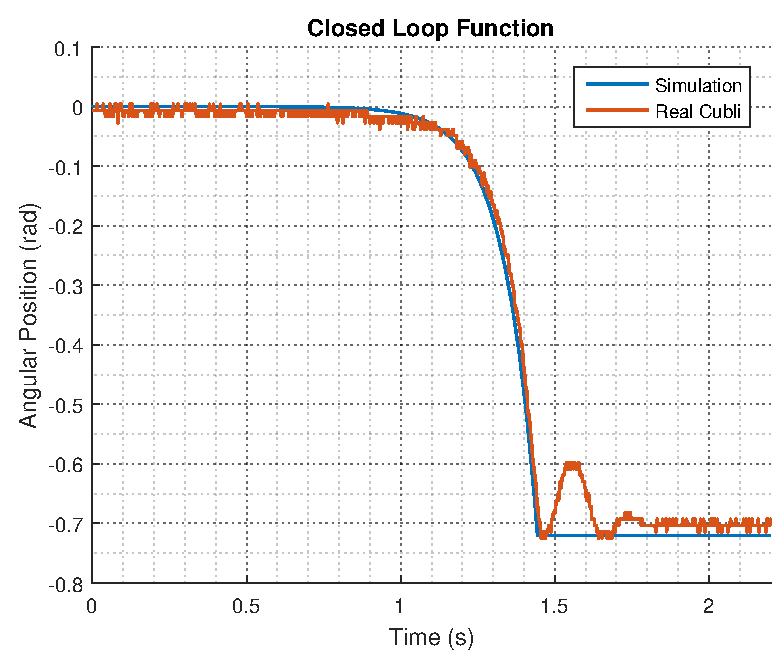
\includegraphics[scale=0.6]{figures/closedLoopResponse}	
	\caption{Behaviour of the closed loop function with a proportional controller of unitary gain}
	\label{closedLoopResponse}
\end{figure}

